\clearpage

\subsection{LEDがてんめつするスクリプト}

かんたんなスクリプトを読み込んでみます。
前の時間と同様に、ファイル→「開く」メニューから「gpio.hsp」を読み込んでから、「F5」キーを押して実行してみましょう。
センサーボードのLEDがてんめつしていたら成功です。うまくいかない人は、となりの友だちか、近くの先生に見てもらいましょう。

\begin{figure}[H]
    \begin{center}
        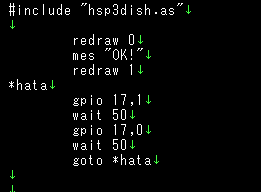
\includegraphics[keepaspectratio,width=8.387cm,height=6.17cm]{text02-img/text02-img023.png}
        \caption{gpio.hspのスクリプト}
    \end{center}
\end{figure}
\noindent
正しく動いたのを確認(かくにん)したらウインドウの「×」ボタンを押して画面を閉じましょう。

\begin{description}
    \item (HSPのルール) 
\end{description}

\begin{description}
    \item スクリプトエディタに打ち込んだ通りに動く
    \item 動かす時は[F5]キーを押す
    \item 確認(かくにん)したらウインドウの「×」ボタンを押して画面を閉じる
\end{description}

スクリプトを見てみましょう。
英単語の後に数字書かれているものが何行も書かれています。
最初はまったく意味がわからないですね。
\vskip\baselineskip
\noindent
最初の行にある

\begin{description}
    \item \#include “hsp3dish.as”
\end{description}

\noindent
は、最初に書いておくおまじないのようなものと考えておいてください。
RaspberryPiを使う時には、最初にこの1行を入れておくことを覚えておきましょう。
% \vskip\baselineskip
HSPのスクリプトは、英文字による「命令」と数字などによる「パラメーター」によって作られています。

\begin{figure}[H]
    \begin{center}
        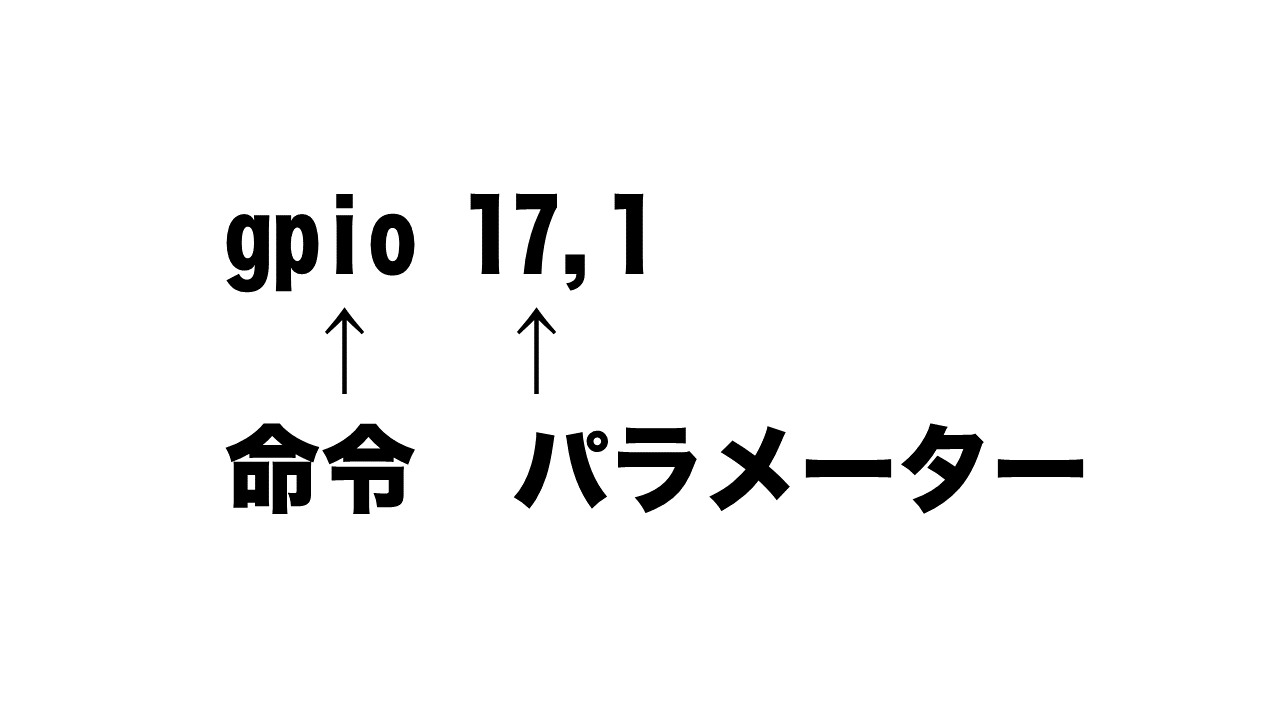
\includegraphics[keepaspectratio,width=8.017cm,height=4.512cm]{text02-img/text02-img024.png}
    \end{center}
\end{figure}

たとえば、「gpio 17,1」という行を見てみましょう。

\begin{description}
    \item (HSPのルール)
\end{description}

\begin{description}
    \item 「gpio」はパソコンに指示を与える「命令」にあたります。
    \item 「命令」の後に、細かい指示の内容を書きます。(パラメーターと呼ぶ)
    \item 「命令」と「パラメーター」の間にはスペース(空白)を入れる
\end{description}
\noindent
つまり、「gpio」が命令、「17」と「1」がパラメーターです。
パラメーターは、「,」によって複数書くことができます。
この「命令」は、コンピューターに何をさせるか、どんな機能を使うかを示しています。
ここで使っている「gpio」は、Raspberry PiのGPIOという端子をせいぎょします。
GPIOは、RaspberryPiの基板からせいぎょすることのできるスイッチのようなものです。
皆さんが使っているセンサーボードの上にあるスイッチやLEDは、GPIOとつながっていて、ON/OFFしたり、スイッチの状態を調べることができます。

\begin{figure}[H]
    \begin{center}
        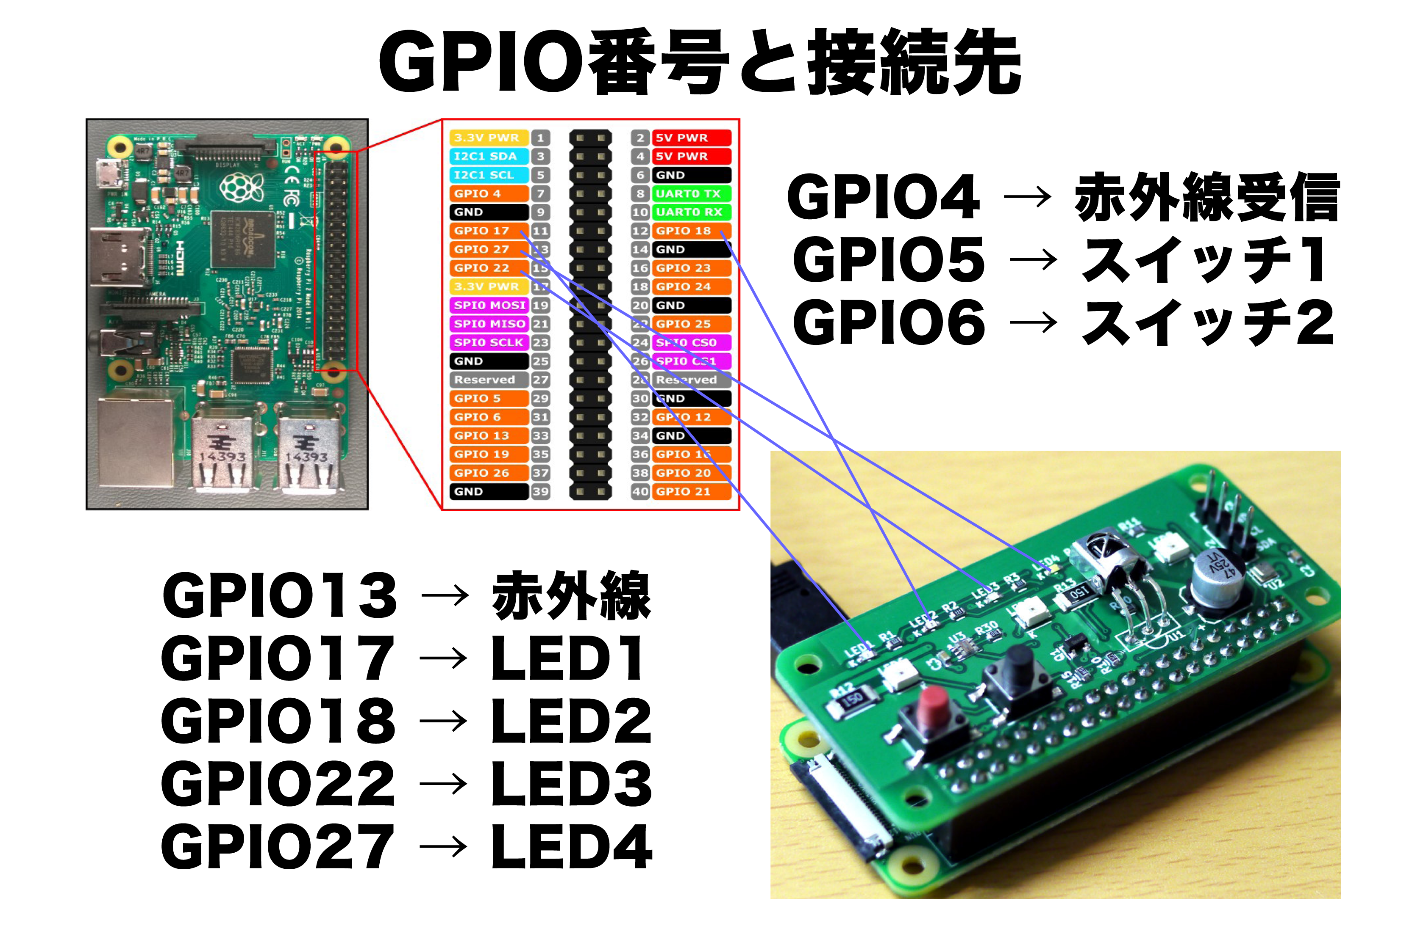
\includegraphics[keepaspectratio,width=12.409cm,height=7.62cm]{text02-img/text02-img025.png}
    \end{center}
\end{figure}

gpioという命令によってLEDのON/OFFがせいぎょできるのかな…と何となく想像できますか?
GPIOのONとOFFのスイッチを切り替えると、センサーボード上のLEDもON/OFFするということになります。

\begin{description}
    \item (HSPのルール)
\end{description}

\begin{description}
    \item gpio命令は、Raspberry PiのGPIOをせいぎょするための命令
    \item gpioの後にスペースに続けて「IO番号」「,(カンマ)」「ON(1)/OFF(0)の値」を書く
\end{description}
\noindent
つまり、「gpio 17,1」という命令は、「GPIO17をONにする」つまりLED1を点灯させることができます。
基板には、LED1〜4までのLEDがとうさいされているので、GPIO17,18,22,27をそれぞれ自由にON/OFFの状態にできるわけです。(赤外線やスイッチについては、また後で説明します。)

スクリプトエディタで、スクリプトを直接修正してみます。
スクリプトの中で「gpio 17,1」と書いてある行を探してから、ためしに下のように他の番号を入れてみましょう。

\begin{description}
    \item gpio 18,1
\end{description}
\noindent
キーボードの入力や、修正のしかたがわからない人は、TAや周りの先生に聞いてみましょう。
修正したら[F5]を押してちゃんと動くか見てみましょう。
おや…LEDが点きっぱなしになりましたね。
実は、LEDがてんめつするためには、ONとOFFの2つを書きます。
つまり、「gpio 17,0」と書かれている部分も修正しなければなりません。

\begin{description}
    \item gpio 18,0
\end{description}
\noindent
に修正して、もう一度[F5]を押しててんめつするか確認(かくにん)してみましょう。

\begin{description}
    \item (HSPのルール)
\end{description}

\begin{description}
    \item 1行目から順番に命令を実行してゆく。
    \item 時間待ちをしたり、くり返したりすることができる。
\end{description}

wait命令は、一定時間停止するための命令です。
パラメーターの数字を修正すれば、てんめつの速度が変わります。

\begin{figure}[H]
    \begin{center}
        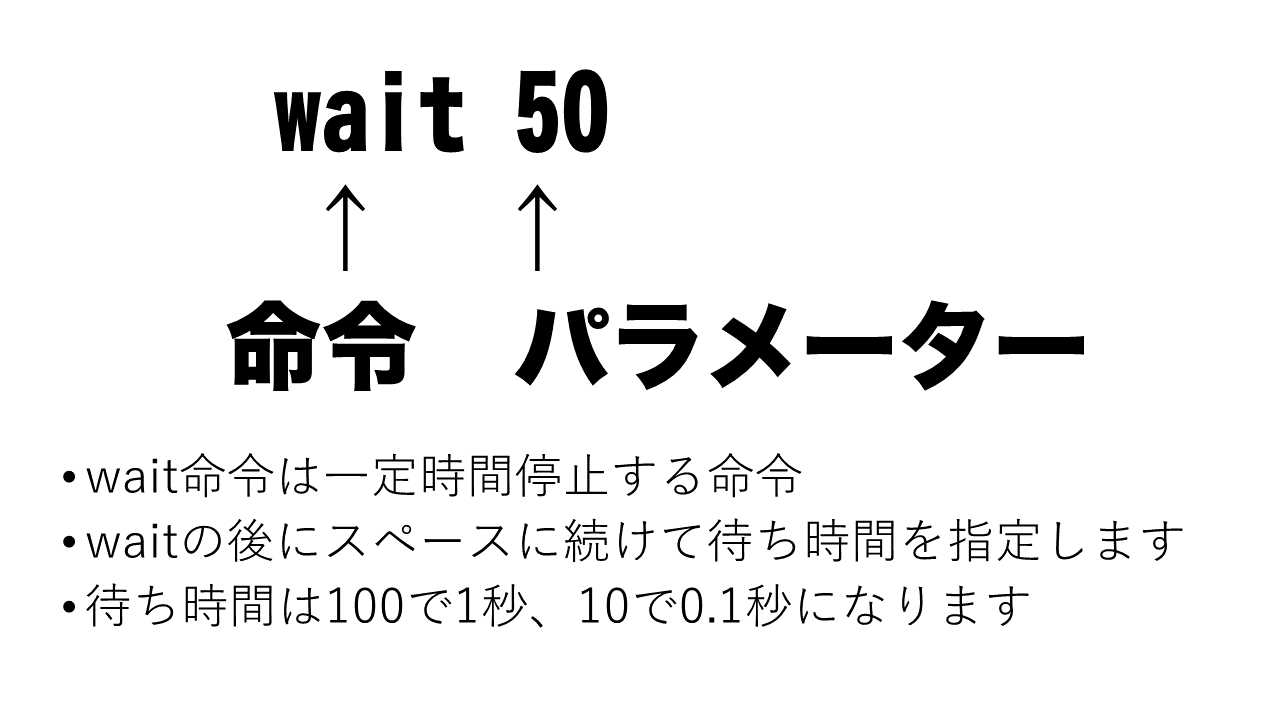
\includegraphics[keepaspectratio,width=10.372cm,height=5.837cm]{text02-img/text02-img026.png}
    \end{center}
\end{figure}
\noindent
このようにコンピューターにわかる言葉、スクリプトを正しく書くことで、その通りに動きます。
どんなに間違ったとしてもコンピューターがこわれることはありません。
うまく動かない時は、どうしてなのか考えてみて、わからない時は質問してみましょう。

